\section{Blocks and Items}\label{sect:block}

\subsection{Blocks}
\begin{frame}{Creating a new NS3 model}
Before introducing Intel HEW on NS3, it is necessary to explain some basic concepts of the NS3 system.
\begin{block}{Creating a new model}
\begin{enumerate}
\item Be familiar with the module layout
\item Create a new module based on the template module
\item Include source and header files into the NS3 system
\item Specify tests and examples of the new module
\item Build and test the new module
\end{enumerate}
\end{block}
\end{frame}

\subsection{Items}
\begin{frame}{Description and Enumerate}
\begin{block}{Requirement: On-line Monitoring System for GSM-R Networks}
\begin{enumerate}
  \item It is crucial to reduce the estimation overhead so that the \alert{on-line monitoring} can be implemented and ensure the realtime reliability.
  \item It is necessary to make \alert{dynamic measurement} due to the feature of propagation environments along the high-speed railway routes.
\end{enumerate}
\end{block}
\begin{itemize}
\item Difficulties:
\begin{description}
  \item[Speed] 250-300km/h for China's high-speed railway;
  \item[Terrains] mountains, viaducts, plains, etc. along the routes;
  \item[Interface] vulnerable to changes of propagation environments;
  \item[Services] the communication may be affected by measurement.
\end{description}
\item Advantages:
\begin{description}
  \item[Flat] the propagation environments are generally flat;
  \item[Fixed] the trajectory and speed of trains are relatively fixed.
\end{description}
\end{itemize}
\end{frame}

\subsection{Footnote Citation}
\begin{frame}{Footnote Citation}
\begin{exampleblock}{Traditional Algorithms on Local Power Estimating}
\begin{itemize}
  \item Lee's method proposed a standard process of local mean power estimation, which is determined in Rayleigh fading channels.\sfcite{lee1985estimate}
  \item Other works are based on confidence degree or ML estimation, but are also analyzed in Rayleigh channels.\sfcite{Ai2009wcsp}
  \item For the estimation of the received signal strength in Rician fading channels, the estimation overhead are usually high for GSM-R.\sfcite{tepedelenlio?lu2001estimation}
  \item The Generalized Lee method does not need a priori knowing of distribution function, but the optimal length of averaging interval is calculated by all the routes of the data with high overhead.\sfcite{Vega2009}
\end{itemize}
\end{exampleblock}
\end{frame}

\section{Figures and Tables}\label{sect:intro}
\subsection{Figures}
\begin{frame}{Mobile Wireless Networks}
\begin{columns}[c]
  \column{2in}
  \begin{figure}
    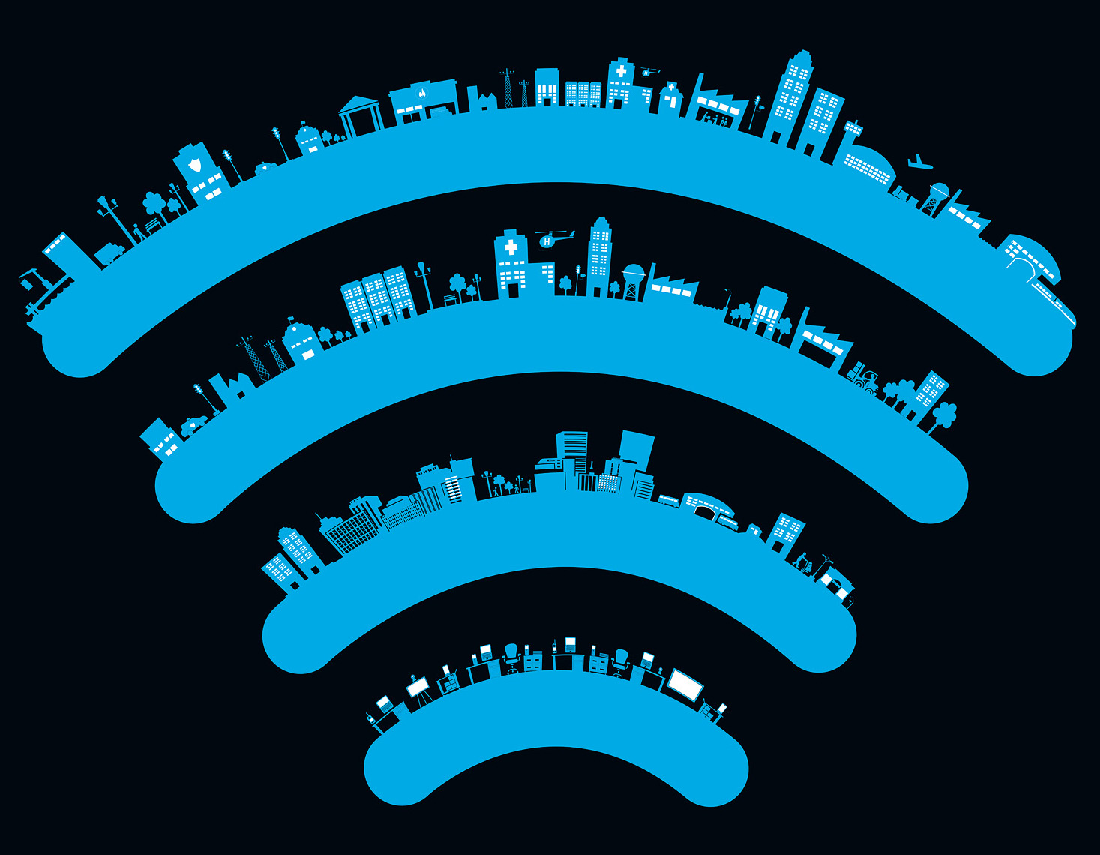
\includegraphics[width=2.0in]{MOT_WNS.pdf}
   \label{connectivity}
  \end{figure}
  \column{2in}
  \begin{figure}
    \includegraphics[width=2.0in]{connectivity.pdf}
  \label{MOT_WNS}
  \end{figure}
\end{columns}
\begin{itemize}
  \item Mobile wireless networks have enjoyed tremendous growth due to the ever-increased demands of mobile applications.
  \item Moreover, the growth is expected to continue unabated with the increasing popularity of ubiquitous smart systems.
  \item The fundamental consideration is how to get suitable trade-off between system reliability and transmission rate?
\end{itemize}
\end{frame}

\subsection{Zooming}
\begin{frame}
\frametitle{Zooming Figures}
\framezoom<1><2>[border](0.5cm,0.5cm)(2cm,1.5cm)
\pgfimage[height=6cm]{whyblue}
%
\includegraphics[height=6cm]{whyblue} is working, too!
Click the border to zoom in.
\end{frame}

\subsection{Tables}
\begin{frame}{Tables}
\begin{block}{Results}
\begin{itemize}
  \item $\Delta d$ is more larger compared to Lee's method when $K=0$, which means the multi-path fading is Rayleigh distributed.
  \item $\Delta d$ may be not so small although $2L$ decreases, for $n<5$ when the terrains gradually become flat until $\nu>10$.
\end{itemize}
\end{block}
\begin{table}[!t]
\renewcommand{\arraystretch}{1}
\centering
\begin{threeparttable}[b]
\caption{Summary of Experiment Results}
\label{summary}
\setlength{\tabcolsep}{4pt}
\scriptsize
\begin{tabular}{c|c||c|c||c|c||c|c||c|c|c}
\hline
\multicolumn{1}{c|}{\multirow{3}{*}{Terrain}} & \multicolumn{1}{c||}{\multirow{3}{*}{$K$(dB)}} & \multicolumn{1}{c|}{\multirow{3}{*}{$\nu$}} & \multicolumn{1}{c||}{\multirow{3}{*}{$\sigma$}} & \multicolumn{1}{c|}{\multirow{3}{*}{$2L(\lambda)$}} & \multicolumn{1}{c||}{\multirow{3}{*}{$N$}} & \multicolumn{1}{c|}{\multirow{3}{*}{$\Delta d(\lambda)$}} & \multicolumn{1}{c||}{\multirow{3}{*}{$\Delta d$(m)}} & \multicolumn{3}{c}{$v_{train}$(km/h)}\\
\cline{9-11}
\multicolumn{1}{c|}{} & \multicolumn{1}{c||}{} & \multicolumn{1}{c|}{} & \multicolumn{1}{c||}{} & \multicolumn{1}{c|}{} & \multicolumn{1}{c||}{} & \multicolumn{1}{c|}{} & \multicolumn{1}{c||}{} & 200 & 250 & 300\\
\cline{9-11}
\multicolumn{1}{c|}{}& \multicolumn{1}{c||}{} & \multicolumn{1}{c|}{} & \multicolumn{1}{c||}{} & \multicolumn{1}{c|}{} & \multicolumn{1}{c||}{} & \multicolumn{1}{c|}{} & \multicolumn{1}{c||}{} & \multicolumn{3}{c}{$\Delta t$(ms)}\\
\cline{1-11}
NLOS\tnote{*}  &  0 &    - & - & 40 & 36 &  1.1 & 0.367 &  2.20 &  1.76 &  1.47\\
\hline
Intensive  &  0 &    0 & 1 & 55 & 15 &  3.7 & 1.222 &  7.33 &  5.86 &  4.89\\
           &  2 &    4 & 2 & 18 & 12 &  1.5 & 0.500 &  3.00 &  2.40 &  2.00\\
           &  4 &  5.6 & 2 &  9 &  9 &  1.0 & 0.333 &  2.00 &  1.60 &  1.33\\
           &  6 &    6 & 3 & 20 &  7 &  2.9 & 0.967 &  5.80 &  4.64 &  3.87\\
           &  8 &   12 & 3 &  8 &  1 &  8.0 & 2.667 & 16.00 & 12.80 & 10.67\\
Open       & 10 &   18 & 4 & 12 &  1 & 12.0 & 4.000 & 24.00 & 19.20 & 16.00\\
\hline
\end{tabular}
\begin{tablenotes}
\item[*] \tiny Caculated by Lee's method in the case of Rayleigh fading
\end{tablenotes}
\end{threeparttable}
\end{table}
\end{frame}

\section{Equations and Codes}
\subsection{Equations}
\begin{frame}{Equations}
\begin{block}{Number of Averaging Samples}
The expectation and variance of $r^2$ can be calculated:

\begin{equation}
    \bar{r^2}=E\left[r^2\right]=\frac{1}{N}E\left[\sum_{i=1}^{N}z_i^2\right]=\frac{\sigma^2}{N}\left(2N+\nu^2\right)
\label{number_mean}
\end{equation}

\begin{equation}
    \sigma_{\bar{r^2}}=D\left[r^2\right]=\frac{1}{N^2}D\left[\sum_{i=1}^{N}z_i^2\right]=\frac{\sigma^4}{N^2}\left(4N+4\nu^2\right)
\label{number_sigma}
\end{equation}
\end{block}
\pause
\uncover<2->
{
\centering
{\Large $\Downarrow$}
\footnotesize
\begin{equation}
\begin{split}
    Q_e=10 \log_{10}\left(\frac{\bar{r^2}+\sigma_{\bar{r^2}}}{\bar{r^2}}\right)&=10 \log_{10}\left(\frac{\frac{\sigma^2}{N}\left(2N+\nu^2\right)+\frac{2\sigma^2}{N}\sqrt{N+\nu^2}}{\frac{\sigma^2}{N}(2N+\nu^2)}\right)\\
    &=10 \log_{10}\left(\frac{2N+\nu^2+2\sqrt{N+\nu^2}}{2N+\nu^2}\right)
\end{split}
\label{Q_e}
\end{equation}
}
\end{frame}

\subsection{Algorithms}
\begin{frame}{Algorithms}
\begin{algorithm}[H]
%\SetAlFnt{\footnotesize}
%\floatname{algorithm}{Procedure}
\renewcommand{\algorithmicrequire}{\textbf{Input:}}
\renewcommand{\algorithmicensure}{\textbf{Output:}}
\caption{GradedM}
\label{alg:graded}
\begin{scriptsize}
\begin{algorithmic}[1]
\Require tx-complete \Comment{packets transmitted event}
\Ensure  rate-index \Comment{rate selection index of HT/GI/MCS}
\While{$txcomplete$} \Comment{defined in \textsf{xmit.c}}
\State{update $txstatus$;}
\State{\Call {DSWA}{$pdrlast,pdrnow$}; \Comment{defined in \textsf{DSWA.c}}}
\State{$rssnow$ $\leftarrow$ \Call{Average}{$rxstatusrss$}; \Comment{defined in \textsf{recv.c}}}
\State{\Call{GradedM}{$pdrnow,rssnow$}; \Comment{defined in \textsf{GradedM.c}}}
\EndWhile
\If{$pdrnow < P_{thrh}$ or $ rssnow < \delta_+$}
\State{$gradedtalbe \gets$ \Call{GradedM}{$pdrnow,rssnow$};} \Comment{defined in \textsf{rc.c}}
\State{$rateindex \gets$ \Call{down-mcs}{$gradedtable$};}
\EndIf
\If{$gradedsens - rssnow > highlimittogray$}
\State{$rateindex \gets$ \Call{up-mcs}{$gradedtable$};}
\EndIf
\State \Return{\{$txstatus,rateindex$\};}
\Function{DSWA}{$pdrlast,pdrnow$}\label{funcDSWA}
  \State{\{$W, \beta$\} $\gets$ \Call{update}{$pdrlast,pdrnow$}}; \Comment{Equation \ref{Q_e}}
  \State{\{$\gamma, \eta$\} $\gets$ \Call{update}{$pdrlast,pdrnow,W,\beta$}; \Comment{Equation \ref{Q_e}}}
  \State{\Return{\{$W,\beta$\}};}
\EndFunction
\end{algorithmic}
\end{scriptsize}
\end{algorithm}
\end{frame}

\subsection{Codes}
\begin{frame}[fragile]
\frametitle{Codes}
The code layout follows the GNU coding standard \sfcite{GNUCoding}.
\begin{lstlisting}
#include "intelhew.h"
void IntelHew::SetHewScenario
{
  switch (scenariotype)
    {
      case RESIDENTIAL:
        StartScenarioResidential(intelHew);
        break;
      default:
        StartScenarioIndoor(intelHew);
        break;
    }
  // Scheduling the CCA only scheduler
  if (wifiMode == INTELHEW_WIFI_CCAOnly_MODE)
    {
      m_sch = CreateObject<CcaOnlyScheduler>();
      Simulator::Schedule(Seconds(0.0),
        &CcaOnlyScheduler::CcaOnlySchedulerInit, m_sch, this);
    }
}
\end{lstlisting}
\end{frame}
